\documentclass[border=10pt]{standalone}
\usepackage{pgfplots}
\pgfplotsset{compat=1.18}

\begin{document}
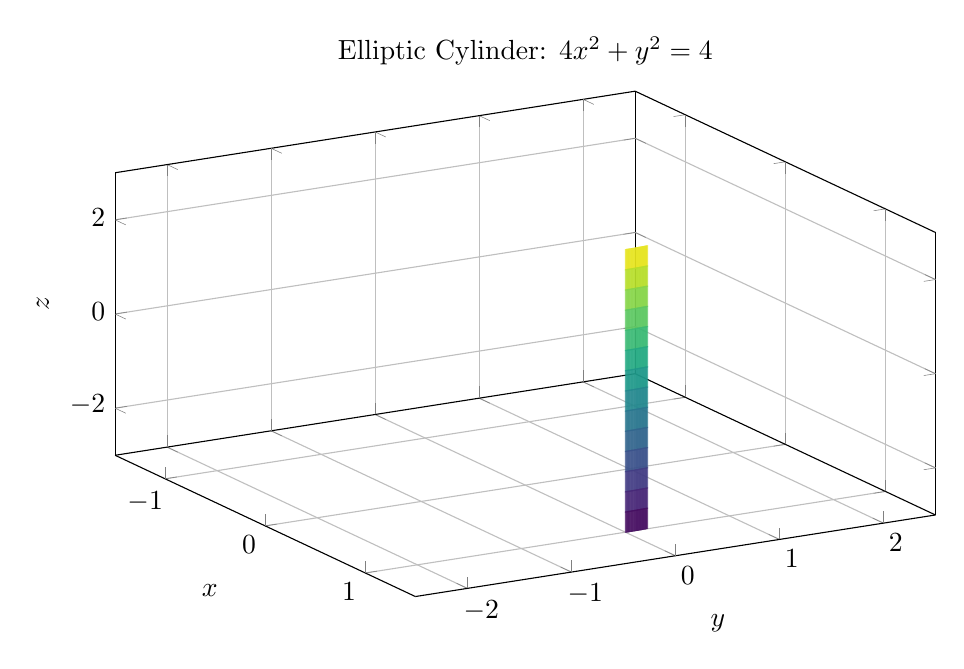
\begin{tikzpicture}
\begin{axis}[
    view={60}{30},
    xlabel={$x$},
    ylabel={$y$},
    zlabel={$z$},
    title={Elliptic Cylinder: $4x^2 + y^2 = 4$},
    colormap/viridis,
    width=12cm,
    height=8cm,
    xmin=-1.5, xmax=1.5,
    ymin=-2.5, ymax=2.5,
    zmin=-3, zmax=3,
    grid=major
]
% Parametric surface using mesh
\addplot3[
    mesh,
    samples=30,
    samples y=15,
    domain=0:6.28,
    y domain=-3:3,
    opacity=0.7
] (
    {cos(x)},
    {2*sin(x)},
    {y}
);
\end{axis}
\end{tikzpicture}
\end{document}